\chapter{ExRORU的实现与实验}\label{cha:experiment}

\section{ExRORU算法的实现}\label{sec:implementation}

\section{实验设计与分析}\label{sec:experiment}
本文实现的ExRORU算法基于jbpt\footnote{\url{https://code.google.com/p/jbpt}}中的CPU抽取WF-net的ExRORU关系并以矩阵形式展现,相关代码已开源共享在Github上\footnote{\url{https://github.com/shudiwsh2009/ExRORU}}。本节介绍ExRORU的实验设计与分析,主要包括有效性实验(将ExRORU与其他算法比较区分过程模型的能力)、性能实验(使用实际模型数据集衡量ExRORU算法的效率)和扩展性实验(衡量ExRORU处理含多并发结构过程模型的能力)等。

\subsection{有效性实验}\label{subsec:effectiveness}
本小节主要展示ExRORU算法强大的刻画过程模型行为语义的能力,并通过在多个模型实例中与第\ref{cha:related_work}中介绍的算法对比,以说明其区分含有不同行为语义的过程模型的能力。

{\heiti 非自由选择结构。}过程模型的任务之间存在间接依赖关系\cite{van2004workflow,van2003workflow,de2003workflow,van2004process},在WF-net上造成了非自由选择结构的存在(即选择关系与同步关系混合的情况)。图\ref{fig:nfc_example_1}中的模型是一个典型的含有非自由选择结构的模型,其中变迁$D$和变迁$E$之间存在非自由选择情形,即他们的执行并不由自身所决定,而是由之前被执行的变迁$A$和变迁$B$决定。具体分析,当在该WF-net的源库所$P_{0}$中放置一个托肯时,变迁$A$和变迁$B$同时被使能,若此时选择执行变迁$A$,则会在库所$_{1}$和库所$P_{2}$中各产生一个托肯;此时只有变迁$C$被使能,其发生之后会消耗库所$P_{1}$的托肯,同时在库所$P_{4}$中产生一个托肯;库所$P_{2}$和库所$P_{4}$各有一个托肯时,显然只有变迁$D$被使能。另一方面,若一开始选择执行变迁$B$,同理可知在变迁$C$发生之后只有变迁$E$被使能。因此,该模型的变迁执行序列只有$\langle A,C,D\rangle$和$\langle B,C,E\rangle$两条。

与之相对的是图\ref{fig:nfc_example_2}中不含有非自由选择结构的模型。与图\ref{fig:nfc_example_1}中的模型相比,该模型少了两个库所和四条边,其中变迁$D$和变迁$E$不存在非自由选择情形,即他们的执行由自身竞争库所$P_{2}$中的托肯所决定。因此,该模型的变迁执行序列有$\langle A,C,D\rangle$、$\langle A,C,E\rangle$、$\langle B,C,D\rangle$和$\langle B,C,E\rangle$四条。

以TAR算法为例,两个模型的TAR集合都是$\{\langle A,C\rangle,\langle C,D\rangle,\langle B,C\rangle,\langle C,E\rangle\}$,显然TAR算法未考虑非自由选择结构蕴含的任务间接依赖关系,所以无法区分这一组模型的行为。本文改进的基础RORU算法是通过任务间关系传递性来抽取因果关系的,然而在图\ref{fig:nfc_example_1}的模型中,变迁$A$与$C$之间的因果关系和变迁$C$与$E$之间的因果关系并不满足传递性,故RORU算法在处理该模型时会出错。

实际上,图\ref{fig:nfc_example_1}的模型只有两个过程流,分别表示为$[A\{C\}D]$和$[B\{C\}E]$(虽然在变迁$A$和变迁$B$后都有并行结构,但是均只有一个分支含有变迁$C$,另一个分支是无变迁分支)。因此,在该模型中,变迁$A$和变迁$D$满足“间接总是因果关系”,即$A\overset{\text{\tiny{IA}}}{\rightarrow}D$;变迁$B$和变迁$E$也满足“间接总是因果关系”,即$B\overset{\text{\tiny{IA}}}{\rightarrow}E$。另一方面,图\ref{fig:nfc_example_2}的模型有4个过程流,分别表示为$[ACD]$、$[ACE]$、$[BCD]$和$[BCE]$,因此在该模型中变迁$A$和变迁$D$满足“间接有时因果关系”,即$A\overset{\text{\tiny{IS}}}{\rightarrow}D$;变迁$B$和变迁$E$也满足“间接有时因果关系”,即$B\overset{\text{\tiny{IS}}}{\rightarrow}E$。两个模型的ExRORU关系矩阵如表\ref{tab:nfc_example}所示,两个模型的行为差异主要体现在变迁$A$与变迁$D$、变迁$E$之间的因果关系和逆因果关系以及变迁$B$与变迁$D$、变迁$E$之间的因果关系和逆因果关系上。因此,ExRORU算法可以检测该组模型之间的差异。

\begin{table}[htbp]
  \centering
  \setlength\tabcolsep{4pt}
  \caption{图\ref{fig:nfc_example}中两个模型的ExRORU矩阵}
  \label{tab:nfc_example}
  \begin{subtable}{1\textwidth}
    \centering
    \caption{图\ref{fig:nfc_example_1}中模型的ExRORU矩阵}
    \label{tab:nfc_example_1}
    \begin{minipage}[b]{0.3\textwidth}
      \centering
      \begin{tabular}{|c|c|c|c|c|c|} \hline
        $\rightarrow$ & $A$ & $B$ & $C$ & $D$ & $E$\\ \hline
        $A$ & $\overset{\text{\tiny{N}}}{\rightarrow}$ & $\overset{\text{\tiny{N}}}{\rightarrow}$ & $\overset{\text{\tiny{DA}}}{\rightarrow}$ & $\overset{\text{\tiny{DA}}}{\rightarrow}$ & $\overset{\text{\tiny{N}}}{\rightarrow}$\\ \hline
        $B$ & $\overset{\text{\tiny{N}}}{\rightarrow}$ & $\overset{\text{\tiny{N}}}{\rightarrow}$ & $\overset{\text{\tiny{DA}}}{\rightarrow}$ & $\overset{\text{\tiny{N}}}{\rightarrow}$ & $\overset{\text{\tiny{DA}}}{\rightarrow}$\\ \hline
        $C$ & $\overset{\text{\tiny{N}}}{\rightarrow}$ & $\overset{\text{\tiny{N}}}{\rightarrow}$ & $\overset{\text{\tiny{N}}}{\rightarrow}$ & $\overset{\text{\tiny{DS}}}{\rightarrow}$ & $\overset{\text{\tiny{DS}}}{\rightarrow}$\\ \hline
        $D$ & $\overset{\text{\tiny{N}}}{\rightarrow}$ & $\overset{\text{\tiny{N}}}{\rightarrow}$ & $\overset{\text{\tiny{N}}}{\rightarrow}$ & $\overset{\text{\tiny{N}}}{\rightarrow}$ & $\overset{\text{\tiny{N}}}{\rightarrow}$\\ \hline
        $E$ & $\overset{\text{\tiny{N}}}{\rightarrow}$ & $\overset{\text{\tiny{N}}}{\rightarrow}$ & $\overset{\text{\tiny{N}}}{\rightarrow}$ & $\overset{\text{\tiny{N}}}{\rightarrow}$ & $\overset{\text{\tiny{N}}}{\rightarrow}$\\ \hline
      \end{tabular}
    \end{minipage}
    \begin{minipage}[b]{0.3\textwidth}
      \centering
      \begin{tabular}{|c|c|c|c|c|c|} \hline
        $\leftarrow$ & $A$ & $B$ & $C$ & $D$ & $E$\\ \hline
        $A$ & $\overset{\text{\tiny{N}}}{\leftarrow}$ & $\overset{\text{\tiny{N}}}{\leftarrow}$ & $\overset{\text{\tiny{N}}}{\leftarrow}$ & $\overset{\text{\tiny{N}}}{\leftarrow}$ & $\overset{\text{\tiny{N}}}{\leftarrow}$\\ \hline
        $B$ & $\overset{\text{\tiny{N}}}{\leftarrow}$ & $\overset{\text{\tiny{N}}}{\leftarrow}$ & $\overset{\text{\tiny{N}}}{\leftarrow}$ & $\overset{\text{\tiny{N}}}{\leftarrow}$ & $\overset{\text{\tiny{N}}}{\leftarrow}$\\ \hline
        $C$ & $\overset{\text{\tiny{DS}}}{\leftarrow}$ & $\overset{\text{\tiny{DS}}}{\leftarrow}$ & $\overset{\text{\tiny{N}}}{\leftarrow}$ & $\overset{\text{\tiny{N}}}{\leftarrow}$ & $\overset{\text{\tiny{N}}}{\leftarrow}$\\ \hline
        $D$ & $\overset{\text{\tiny{DA}}}{\leftarrow}$ & $\overset{\text{\tiny{N}}}{\leftarrow}$ & $\overset{\text{\tiny{DA}}}{\leftarrow}$ & $\overset{\text{\tiny{N}}}{\leftarrow}$ & $\overset{\text{\tiny{N}}}{\leftarrow}$\\ \hline
        $E$ & $\overset{\text{\tiny{N}}}{\leftarrow}$ & $\overset{\text{\tiny{DA}}}{\leftarrow}$ & $\overset{\text{\tiny{DA}}}{\leftarrow}$ & $\overset{\text{\tiny{N}}}{\leftarrow}$ & $\overset{\text{\tiny{N}}}{\leftarrow}$\\ \hline
      \end{tabular}
    \end{minipage}
    \begin{minipage}[b]{0.3\textwidth}
      \centering
      \begin{tabular}{|c|c|c|c|c|c|} \hline
        $\leftarrow$ & $A$ & $B$ & $C$ & $D$ & $E$\\ \hline
        $A$ & $\nparallel$ & $\nparallel$ & $\nparallel$ & $\nparallel$ & $\nparallel$\\ \hline
        $B$ & $\nparallel$ & $\nparallel$ & $\nparallel$ & $\nparallel$ & $\nparallel$\\ \hline
        $C$ & $\nparallel$ & $\nparallel$ & $\nparallel$ & $\nparallel$ & $\nparallel$\\ \hline
        $D$ & $\nparallel$ & $\nparallel$ & $\nparallel$ & $\nparallel$ & $\nparallel$\\ \hline
        $E$ & $\nparallel$ & $\nparallel$ & $\nparallel$ & $\nparallel$ & $\nparallel$\\ \hline
      \end{tabular}
    \end{minipage}
  \end{subtable}

  \begin{subtable}{1\textwidth}
    \vspace{1em}
    \centering
    \caption{图\ref{fig:nfc_example_2}中模型的ExRORU矩阵}
    \label{tab:nfc_example_2}
    \begin{minipage}[b]{0.3\textwidth}
      \centering
      \begin{tabular}{|c|c|c|c|c|c|} \hline
        $\rightarrow$ & $A$ & $B$ & $C$ & $D$ & $E$\\ \hline
        $A$ & $\overset{\text{\tiny{N}}}{\rightarrow}$ & $\overset{\text{\tiny{N}}}{\rightarrow}$ & $\overset{\text{\tiny{DA}}}{\rightarrow}$ & $\overset{\text{\tiny{DS}}}{\rightarrow}$ & $\overset{\text{\tiny{DS}}}{\rightarrow}$\\ \hline
        $B$ & $\overset{\text{\tiny{N}}}{\rightarrow}$ & $\overset{\text{\tiny{N}}}{\rightarrow}$ & $\overset{\text{\tiny{DA}}}{\rightarrow}$ & $\overset{\text{\tiny{DS}}}{\rightarrow}$ & $\overset{\text{\tiny{DS}}}{\rightarrow}$\\ \hline
        $C$ & $\overset{\text{\tiny{N}}}{\rightarrow}$ & $\overset{\text{\tiny{N}}}{\rightarrow}$ & $\overset{\text{\tiny{N}}}{\rightarrow}$ & $\overset{\text{\tiny{DS}}}{\rightarrow}$ & $\overset{\text{\tiny{DS}}}{\rightarrow}$\\ \hline
        $D$ & $\overset{\text{\tiny{N}}}{\rightarrow}$ & $\overset{\text{\tiny{N}}}{\rightarrow}$ & $\overset{\text{\tiny{N}}}{\rightarrow}$ & $\overset{\text{\tiny{N}}}{\rightarrow}$ & $\overset{\text{\tiny{N}}}{\rightarrow}$\\ \hline
        $E$ & $\overset{\text{\tiny{N}}}{\rightarrow}$ & $\overset{\text{\tiny{N}}}{\rightarrow}$ & $\overset{\text{\tiny{N}}}{\rightarrow}$ & $\overset{\text{\tiny{N}}}{\rightarrow}$ & $\overset{\text{\tiny{N}}}{\rightarrow}$\\ \hline
      \end{tabular}
    \end{minipage}
    \begin{minipage}[b]{0.3\textwidth}
      \centering
      \begin{tabular}{|c|c|c|c|c|c|} \hline
        $\leftarrow$ & $A$ & $B$ & $C$ & $D$ & $E$\\ \hline
        $A$ & $\overset{\text{\tiny{N}}}{\leftarrow}$ & $\overset{\text{\tiny{N}}}{\leftarrow}$ & $\overset{\text{\tiny{N}}}{\leftarrow}$ & $\overset{\text{\tiny{N}}}{\leftarrow}$ & $\overset{\text{\tiny{N}}}{\leftarrow}$\\ \hline
        $B$ & $\overset{\text{\tiny{N}}}{\leftarrow}$ & $\overset{\text{\tiny{N}}}{\leftarrow}$ & $\overset{\text{\tiny{N}}}{\leftarrow}$ & $\overset{\text{\tiny{N}}}{\leftarrow}$ & $\overset{\text{\tiny{N}}}{\leftarrow}$\\ \hline
        $C$ & $\overset{\text{\tiny{DS}}}{\leftarrow}$ & $\overset{\text{\tiny{DS}}}{\leftarrow}$ & $\overset{\text{\tiny{N}}}{\leftarrow}$ & $\overset{\text{\tiny{N}}}{\leftarrow}$ & $\overset{\text{\tiny{N}}}{\leftarrow}$\\ \hline
        $D$ & $\overset{\text{\tiny{DS}}}{\leftarrow}$ & $\overset{\text{\tiny{DS}}}{\leftarrow}$ & $\overset{\text{\tiny{DA}}}{\leftarrow}$ & $\overset{\text{\tiny{N}}}{\leftarrow}$ & $\overset{\text{\tiny{N}}}{\leftarrow}$\\ \hline
        $E$ & $\overset{\text{\tiny{DS}}}{\leftarrow}$ & $\overset{\text{\tiny{DS}}}{\leftarrow}$ & $\overset{\text{\tiny{DA}}}{\leftarrow}$ & $\overset{\text{\tiny{N}}}{\leftarrow}$ & $\overset{\text{\tiny{N}}}{\leftarrow}$\\ \hline
      \end{tabular}
    \end{minipage}
    \begin{minipage}[b]{0.3\textwidth}
      \centering
      \begin{tabular}{|c|c|c|c|c|c|} \hline
        $\leftarrow$ & $A$ & $B$ & $C$ & $D$ & $E$\\ \hline
        $A$ & $\nparallel$ & $\nparallel$ & $\nparallel$ & $\nparallel$ & $\nparallel$\\ \hline
        $B$ & $\nparallel$ & $\nparallel$ & $\nparallel$ & $\nparallel$ & $\nparallel$\\ \hline
        $C$ & $\nparallel$ & $\nparallel$ & $\nparallel$ & $\nparallel$ & $\nparallel$\\ \hline
        $D$ & $\nparallel$ & $\nparallel$ & $\nparallel$ & $\nparallel$ & $\nparallel$\\ \hline
        $E$ & $\nparallel$ & $\nparallel$ & $\nparallel$ & $\nparallel$ & $\nparallel$\\ \hline
      \end{tabular}
    \end{minipage}
  \end{subtable}
\end{table}

{\heiti 多关系。}如本文算法所述,过程模型中的两个变迁$X$和$Y$之间可能存在多种类型的关系。如图\ref{fig:multi_relation}所示,图\subref{fig:multi_relation_petri}是含有多关系变迁对的WF-net示例,图\subref{fig:multi_relation_cpu}是其对应的CPU,其中变迁$A$和变迁$D$可以同时满足因果关系和并行关系。具体分析,当在该WF-net的源库所$P_{0}$中放置一个托肯时,变迁$I$被使能,当其被执行后,会在库所$P_{1}$和库所$P_{2}$中各产生一个托肯;接下来触发变迁$A$,则此时库所$P_{2}$和库所$P_{3}$中各有一个托肯,变迁$B$、变迁$C$和变迁$E$同时被使能;在这种情况下,若选择触发变迁$E$则会同时消耗两个托肯,并在库所$P_{4}$和库所$P_{5}$中各产生一个托肯,变迁$B$和变迁$C$都被跳过,然而若触发变迁$B$或者变迁$C$,则会夺走变迁$E$输入库所中的托肯使其不能被触发。

从CPU中可知该模型共有两个过程流,分别表示为$[I\{AC,BD\}O]$和$[I\{A\}E\{D\}O]$,由ExRORU算法得到变迁$A$和变迁$D$满足“间接有时因果关系”,即$A\overset{\text{\tiny{IS}}}{\rightarrow}D$;同时它们满足“有时并行关系”,即$A\Uparrow D$。

\begin{figure}[htbp]
  \centering
  \begin{subfigure}{1\textwidth}
    \centering
    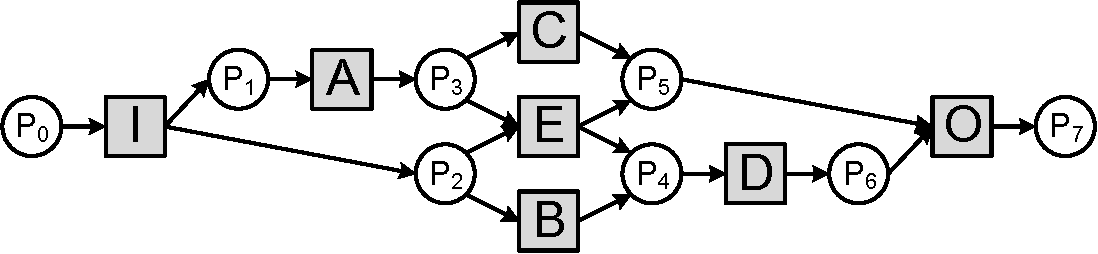
\includegraphics[width=0.7\textwidth]{multi_relation_petri}
    \caption{含有多关系变迁对的WF-net}
    \label{fig:multi_relation_petri}
  \end{subfigure}
  \begin{subfigure}{1\textwidth}
    \vspace{1em}
    \centering
    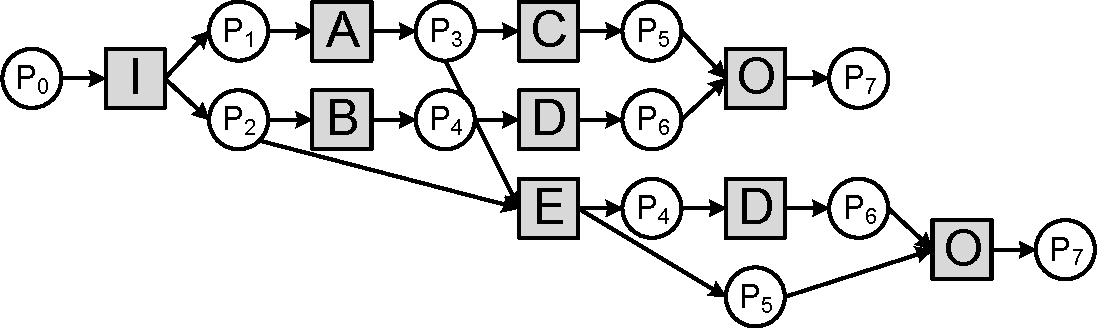
\includegraphics[width=0.7\textwidth]{multi_relation_cpu}
    \caption{图\subref{fig:multi_relation_petri}中WF-net对应的CPU}
    \label{fig:multi_relation_cpu}
  \end{subfigure}
  \caption{含有多关系变迁对的模型示例}
  \label{fig:multi_relation}
\end{figure}

绝大多数算法如BP、TAR等都不能识别变迁对之间多关系的存在,因为它们将每对变迁之间的关系定义为单独一种,因此这些算法也无法准确地刻画过程模型的行为语义从而不能有效地区分含有多关系变迁对的模型。虽然RORU算法允许一对变迁之间存在多种关系,但是它并没有对一个变迁在CPU中对应多个事件的情况作处理。根据RORU的计算方法,CPU中的每个事件都被当作独立事件参与事件间RORU关系的计算,RORU并没有提及如何将多个对应事件与其他事件的关系折叠回原始变迁对之间的RORU关系。例如,在图\ref{fig:multi_relation}的模型中,RORU无法确定变迁$D$(变迁$D$在图\ref{fig:multi_relation_cpu}的CPU中有两个对应事件,变迁$O$也一样)和其他变迁之间的关系。

\section{本章小结}